\section{Introduction}

The Paris Climate Change Conference (COP 21) \parencite{agreement2015unfccc, agreement2015paris} was tasked to address the greatest challenge ever faced by the world - Global Warming (Figure \ref{fig:RNN_annual_carbon_data}). The principal target of this conference was to adopt a new climate agreement to limit global warming to well below $2^{\circ}$C, as compared to pre-industrial levels. All the participating nations submitted national plans to achieve this target in the next few decades and identified options that may help to reduce anthropogenic greenhouse gas (GHG) emissions. One of the largest contributors to GHG emissions is the transportation sector. This has been shown in a study performed in the USA (U.S. Greenhouse Gas Emissions and Sinks 1990–2018) \parencite{epa2018inventory}, under the United Nations Framework Convention on Climate Change (UNFCCC), where it was found that the transportation sector accounted for the largest portion (28\%) of total U.S. GHG emissions in 2018, followed by electricity generation as shown in Figure \ref{fig:RNN_US_GHG_emissions_sectors}. The worldwide contribution of the transportation sector towards global $CO_2$ emissions is at 14\%, with 95\% of the worlds' transportation energy coming from burning fossil fuels, especially gasoline and diesel.  

\begin{figure}[h!]
    \centering
    \includegraphics[width= \textwidth]{Figures/Chp_RNN/annual-carbon-data.png}
    \caption{Annual (a) $CO_2$ emission (b) Global land-sea temperature increase relative to 1961-1990 average temperature. Data from \parencite{friedlingstein2019global}.}
    \label{fig:RNN_annual_carbon_data}
\end{figure}

\begin{figure}[h!]
    \centering
    \includegraphics[width=0.65\textwidth]{Figures/Chp_RNN/US_GHG_Emissions_by_Sector.png}
    \caption{US GHG Emissions by Sector}
    \label{fig:RNN_US_GHG_emissions_sectors}
\end{figure}

\begin{figure}[h!]
    \centering
    \includegraphics[width=0.75\textwidth]{Figures/Chp_RNN/US_Transportation_Sector_GHG_Emissions_by_Source.png}
    \caption{US Transportation Sector GHG Emissions by Source}
    \label{fig:RNN_US_Transportation_Sector_GHG_Emissions_by_Source}
\end{figure}

Cars, trucks, commercial aircraft, and railroads, among other sources, all contribute to transportation sector emissions. In the same study, \parencite{epa2018inventory}, it was also observed that the trend from 1990 to 2018 (for the USA) shows that GHG emissions in the transportation sector increased more in absolute terms than any other sector (i.e. electricity generation, industry, agriculture, residential, commercial), largely due to increased demand for travel and personal ownership of vehicles.  Within the transportation sector, light-duty vehicles (including passenger cars and light-duty trucks) were by far the largest category, with 59\% of GHG emissions, while medium- and heavy-duty trucks made up the second-largest category, with 23\% of emissions, a combined share of 82\% as shown in  Figure \ref{fig:RNN_US_Transportation_Sector_GHG_Emissions_by_Source}. The greenhouse gas pollution that causes global warming comes from numerous sources ($CO_2, CH_4, N_2O \text{ and various } HFCs$). Although automobiles release most of the GHG, the main contribution comes from the carbon dioxide ($CO_2$) emitted as the engine burns fuel. 

To reduce the GHG emissions, governments and car manufacturers around the world are setting ambitious targets of ending the sale of combustion engine-based cars in the not too distant future. Thus, targeting the 82\% share of carbon emissions from the transportation sector, agencies such as the European Environment Agency (EEA) are also designing strict guidelines and placing heavy emission premiums to limit the $CO_2$ emissions \parencite{european2016monitoring, european2015evaluating}. With a similar focus on reducing carbon emissions, the US Department of Energy \parencite{yang2015comparative} has also encouraged researchers and automotive manufacturers to design highly efficient drivetrains for variable-speed drives such as those for hybrid and electric vehicles (HEVs). HEVs serve as an alternative to fossil fuel-based vehicles and have become popular in recent years. They offer a chance for a more environmentally-friendly mode of transportation and an increasingly viable solution to the global pollution crisis. The popularity of HEVs is due to other factors too. A study from the University of Michigan's Transportation Research Institute \parencite{sivak2018relative} found that electric vehicles cost less than half as much to operate as gas-powered cars. 

This serves as a massive motivation to develop techniques that can help improve the efficiency of electric vehicles so that they become even more popular and efficient. One of the most effective graphical ways to describe the performance of an electric machine is through a performance map. This chapter is dedicated to finding novel statistical solutions to generate performance maps such as efficiency and power factor maps. Although only two types of electric motors are considered, the techniques discussed in this chapter can easily be adapted for all kinds of electric machines.

\section{Literature survey}

The main component of an electric drivetrain is the electric motor. Electric motors used in the majority of industrial applications operate at one or a few predefined operating points. As such motors designed for such industrial usage are optimized for specific operating points and the performance is well defined. Additionally, many machines were designed to operate at either dc or a fixed frequency and voltage, e.g. 60Hz, 110volts. The development of power electronics; the electrification of many systems; and the need to operate efficiently over an entire performance envelope rather than just at one point; have significantly changed the design targets of an electric motor. At the same time, motors used in the field of Electric Vehicles and Hybrid Electric Vehicles are expected to operate efficiently over the entire torque-speed range. Further, the machine is designed to account for frequent start/stop and high acceleration and deceleration. To analyze a motor's performance, it has to be studied at all possible torque-speed combinations within the motor's operating range.

\begin{comment}
Source: 
In most industrial applications of motor drives, motors operate at one or a few predefined operating points. Therefore the motor can be optimized to give the best performance at these specific points, and the efficiency of the system is well defined. However, in propulsion applications, the motor is used over the entire torque/speed range. The motor must be designed for frequent start/stop, and high acceleration and deceleration rates. (meaning high torque output for the entire speed range) [1]. Hence, the motor needs high torque density and efficiency at all speeds [2]. Also, the motor drive needs high controllability, steady-state accuracy, and good transient performance [3]–[4][5]. Therefore the performance characteristic of a propulsion motor must be quite different from the industrial motor drive. The motor has to be studied at all possible torque/speed combinations within the motor's operating envelope.
\end{comment}

For a specific drive configuration (battery, inverter, modulation scheme), an electric motor such as the interior permanent magnet (IPM) machine can operate flexibly at different speed and torque points with high-efficiency levels when compared to an internal combustion engine. Typically, these points are represented by an efficiency map as shown in Figure \ref{fig:RNN_Fig-0}. Projecting onto the 2-D plane of speed and torque, the efficiency map consists of varying efficiency levels in different regions. The peak torque is constrained by the motor’s thermal limit, while the maximum speed depends on the rotor’s mechanical structure. The benefit of an efficiency map is for vehicle dynamic simulations, as in \parencite{mahmoudi2015efficiency}, to predict an HEV’s range (or total energy usage) in an urban or highway setting.

\begin{figure}[h!]
    \centering
    \includegraphics[width=0.85\textwidth]{Figures/Chp_RNN/Fig 0.png}
    \caption{Efficiency map of the 2010 Toyota Prius IPM motor \parencite{mahmoudi2015efficiency}.}
    \label{fig:RNN_Fig-0}
\end{figure}

Finding such a map, however, for a given motor design is computationally expensive. The generation of a performance map such as efficiency, power factor, etc., can require significant computation, extending from hours to even days to run finite element (FE) simulations for all operating points and this means that it is difficult to include this information in the early stages of the design process. To tackle this computational burden, related works on designing electric traction motors consider multiple operating points (e.g. rated, peak, or max speed) using surrogate-based optimization to ensure that the designed motor is optimized with respect to different operating conditions \parencite{silva2017multiple}. While this methodology can provide optimal solutions, it is difficult to determine how changing a motor parameter can affect the location of the high-efficiency regions in an efficiency map. However, the performance map itself could be described as a response surface representing the impact of changes in excitation, geometry, and materials on the particular performance parameter over the entire operational envelope. As such, it could be a candidate for a machine learning approach provided that issues such as generalization of the knowledge and the ability to transfer learning between scenarios can be resolved. Having the capability to predict this map reasonably quickly, e.g. in seconds, for use in motor design and optimization as well as in sensitivity analysis will be a significant improvement over the present method.

Recently, deep neural networks (DNNs) have gained popularity in the field of computational electromagnetics, since they can provide relatively accurate solutions in a reasonably short time compared to physics-based simulations. Examples include topology optimization of electric motors \parencite{asanuma2020transfer, barmada2020deep} and performance prediction of motor drives (refer Chapter \ref{chapter:2_CNN}). Such approaches employ data-driven, deep neural networks to approximate the output performance that was derived from the solution of FE solvers.

This chapter explores different architectures and techniques to develop a suitable DL surrogate model for predicting a performance map for different motors. Based on the investigations, this work suggests guidelines for designing a Deep Learning (DL) surrogate using supervised learning. Once the optimal architecture has been identified, the focus will shift to reduce the data and computational requirements associated with supervised learning. 
This chapter aims to extend DL-based surrogate modeling and the content and structure of the chapter are summarized as follows: Section \ref{RNN:3_dataCollection} starts with the setup of the supervised learning task by describing the data collection process. Next in Section \ref{RNN:4_Neural_networks}, the problem description for supervised learning is identified and relevant requirements of the model architecture are discussed. Throughout Section \ref{RNN:5_Results_Discussion}, the results obtained with different supervised task approaches are compared and discussed, before a Bayesian learning approach is used to address the issue of uncertainty in the trained networks. This will conclude the cold start supervised learning task of a performance map estimation. 

From Section \ref{RNN:7_TL_methodology} onwards, the trained networks are extended to train and predict performance maps for a new geometry. This will involve the discussion of a transfer learning strategy and performance analysis in Section \ref{RNN:9_Results_TL}. 


\begin{comment}
\begin{figure}
    \centering
    \includegraphics[width=\textwidth]{Figures/Chp_RNN/Fig 2.png}
    \caption{Caption}
    \label{fig:my_label}
\end{figure}

\end{comment}

\section{Data Collection}\label{RNN:3_dataCollection}

The procedure for efficiency map calculation is given below and shown in Figure \ref{fig:RNN_Fig-1_flowchart_effMaps}, which is based on \cite{mohammadi2017computational}. For a given motor geometry, material and simulation parameters (drive, excitation, time steps), electromagnetic FE simulations using \cite{mentor_motorsolve} are run at different dq currents to obtain the dq flux linkages for characterization in Stage 1. Then, these 9 dq flux linkages points are used to construct flux linkage maps ($\lambda_d,\lambda_q$) as functions of the dq currents using 2nd-degree polynomials. Next in Stage 2, different control strategies, namely the Maximum-Torque-Per-Ampere, Flux Weakening, and Maximum-Torque-Per-Volt, are used to find optimal excitation conditions ($I_s^*,\gamma^*$) for every motor speed $N^*$. In Stage 3, these points are used in FE simulations to compute the values of the electromagnetic torque $T_{em}^*$ and efficiency $\eta^*$. The final ($N^*,T_{em}^*,\eta^*$) points are then post-processed and interpolated to generate an efficiency map in Stage 4.

\begin{figure}[h!]
    \centering
    \includegraphics[width=0.85\textwidth]{Figures/Chp_RNN/Fig 1.png}
    \caption{Flowchart of the process for calculating efficiency maps.}
    \label{fig:RNN_Fig-1_flowchart_effMaps}
\end{figure}

To predict the efficiency map for a given motor geometry, a large dataset of design variations, motor geometric images, and efficiency maps is required. Latin Hypercube sampling \parencite{mckay2000comparison} was used to populate a design space of 2900 samples of a 24-slot 4-pole parameterized IPM motor displayed in Figure \ref{fig:RNN_Fig-2_IPMMotor}. A variation of ±50\% was set on each of the reference design parameters (shown in Table \ref{tab:RNN-1_IPMMotor}). Of these samples, 2500, 200, and 200 were randomly partitioned for the training, validation, and test sets. For each motor sample around 120 FE simulations were used for Stages 1 and 3.

\vspace{14pt}

\begin{minipage}{0.95\textwidth}
  \begin{minipage}[b]{0.4\textwidth}
    \centering
    \includegraphics[width=\textwidth]{Figures/Chp_RNN/Fig 2.png}
    \captionof{figure}{Parametrized Motor Geometry - IPM Motor.}
    \label{fig:RNN_Fig-2_IPMMotor}
  \end{minipage}
  \hfill
  \begin{minipage}[b]{0.55\textwidth}
    \centering
    \begin{tabular}{||c||}\hline
      Independent Parameters \\ \hline
        24 slots \hspace{20pt} 4 poles \\
        33.33 A_{rms} \hspace{10pt} 400 V_{dc} \\ \hline \hline
    \end{tabular}
    \centering
    \begin{tabular}{||c|c||c|c||}\hline
      Parameter & Value & Parameter & Value \\ \hline \hline
        $X_1$ & 18 mm & $X_7$ & 50 mm\\
        $X_2$ & 5.8 mm & $X_8$ & 18 mm\\
        $X_3$ & 3 mm & $X_9$ & 4 mm\\
        $X_4$ & 1 mm & $X_{10}$ & 15 mm\\
        $X_5$ & 1 mm & $X_{11}$ & 45^{\circ}\\ 
        $X_6$ & 100 mm & $X_{12}$ & 1.5 mm\\\hline
      \end{tabular}
      \captionof{table}{Dependent \& Independent Parameters of the reference design.}
      \label{tab:RNN-1_IPMMotor}
    \end{minipage}
\end{minipage}

\section{Neural Networks} \label{RNN:4_Neural_networks}
Due to the high cost of generating an efficiency map from detailed FE computations, Stages 1 and 3 in Figure \ref{fig:RNN_Fig-1_flowchart_effMaps} which usually involves FE simulations, are targeted as candidates for DL models. The first model is based on an Artificial Neural Network-Convolutional Neural Network (ANN-CNN) architecture and acts as a surrogate to Stage 1 for ‘Flux Linkage Calculation’ shown in Figure \ref{fig:RNN_Fig-1_flowchart_effMaps}. Similarly, a second network discussed later, learns the behavior of the ‘Torque and Efficiency Calculation’ FE simulations in Stage 3 of Figure \ref{fig:RNN_Fig-1_flowchart_effMaps}. This model is based on a combined CNN-Recurrent Neural Network (RNN) architecture. Note that the terms feedforward network and ANN are used interchangeably in this work.

\begin{figure}[h!]
    \centering
    \includegraphics[width=\textwidth]{Figures/Chp_RNN/Fig 3_mod.png}
    \caption{Neural network-based flux linkage prediction.}
    \label{fig:RNN_Fig-3_neuralnet_fluxLinkage}
\end{figure}

\subsection{Modular network approach}\label{RNN:4.1_Modular_nw_approach_theory}

% Compumag
The aim of the model in Figure \ref{fig:RNN_Fig-3_neuralnet_fluxLinkage} is to predict the values of dq flux linkages (Stage 1, Figure \ref{fig:RNN_Fig-1_flowchart_effMaps}), necessary for characterizing a motor drive. This model consists of three sub-networks. The first takes the CAD geometry, which is parametrized to change dimensions to build a design space consisting of 2900 different designs (samples), along with the information of material distribution in the form of a pixelated image as input to a CNN. In parallel, the current excitation ($I_s,\gamma$) represented as a 1-D vector is fed to the first feedforward network. After the information passes through a series of hidden layers on both sides of the network (ANN and CNN), the hidden output from the CNN is flattened and merged with the hidden vector of the first ANN, which is fed to the second feedforward network, which then predicts the target dq flux linkages. 
The flux linkage map, obtained by interpolating the predicted dq flux linkage values, is used for calculating the optimal control values ($N^*,I_s^*,\gamma*$) in Stage 2. These points along with the pixelated input of CAD geometry and material distribution, are used as input for the Stage 3 surrogate model, as represented in Figure \ref{fig:RNN_Fig-4_RNN_EffMaps} to predict the corresponding efficiency ($\eta^*$) values. However, due to the different torque-speed range of various designs, the output length depends on the number of inputs. This means that a model architecture suited to handle variable input sequence length is required. Although an efficiency map is represented on a 2D map, the torque-speed points can be represented in the form of a 1D sequence. The conversion of a 2D map to a 1D sequence can be done in many ways - row first, column first, or in any random order. The architecture for performance should be independent of the order of the sequence and should rather be able to identify the spatial relation over a large separation over the sequence of the input. For these requirements, a popular DL algorithm for such sequence-to-sequence modeling is based on using RNNs with an attention mechanism to handle long-term dependencies as in Figure \ref{fig:RNN_Fig-4_RNN_EffMaps} (a).  This part of the model is called the ‘Encoder’. Finally, a dense time distributed layer in Figure \ref{fig:RNN_Fig-4_RNN_EffMaps} (b) accumulates information from all the sub-networks and works as a decoder to predict the target in the form of a sequence of efficiency values.

\begin{figure}[h!]
    \centering
    \includegraphics[width=\textwidth]{Figures/Chp_RNN/Fig 4.png}
    \caption{Network architecture: (a) RNN with attention mechanism, (b) prediction from time distributed feedforward layers.}
    \label{fig:RNN_Fig-4_RNN_EffMaps}
\end{figure}

There are five inputs fed to the sequence-based model: the excitation ($N^*,I_s^*,\gamma^*$) and torque values ($T_{em}^*$) along with the base speed ($N_{base}^*$), for all the points where efficiency values are to be calculated, as displayed in Figure \ref{fig:RNN_Fig-4_RNN_EffMaps} (a). An RNN cell consists of hidden memory elements which are responsible for encoding long-term dependencies \parencite{graves2013speech} in the input sequence, shown with the dotted arrow in Figure \ref{fig:RNN_Fig-4_RNN_EffMaps} (a). Once the RNN has seen all the input sequence, the encoded hidden information is referred to as the context. This context vector is initialized with information related to the motor geometry, provided either as geometric parameters or through a CNN as in Figure \ref{fig:RNN_Fig-4_RNN_EffMaps} (a), and encodes input information (geometric parameters, excitation, torque) relevant for the prediction. In brief, this vector tries to summarize the global information for a design sample from the inputs in a single abstract representation. 

Even though efficiency maps can be predicted with just the context and encoder hidden vector, there is an information loss which leads to poor performance. This occurs when all the input data and motor geometric information is encoded into a potentially long sequence ($ \sim 120-170$). To mitigate this issue, we introduce an attention mechanism \parencite{vaswani2017attention} in Figure \ref{fig:RNN_Fig-4_RNN_EffMaps} (a). The importance of this attention mechanism can be attributed to the smooth regions of an efficiency map. For an intuitive understanding, the neighboring regions in the map can contribute to the prediction as they tend to have similar values especially in the regions of high efficiency. Thus, the closer the neighbor is to the point of prediction, the higher the voting power (i.e. attention) it gets. The calculation of attention can be costly as the model needs to compute the attention value for each combination of input and output sequence elements. As for the operation in the attention layer, the input sequence is assembled and is compared with the information captured by the encoder sequence to generate a corresponding score. As an example, assume that an attention score ($a_{32}$) is large, then the second encoder output state will get a lot of attention while predicting the value of efficiency for sequence step 3. This can be visualized in Figure \ref{fig:RNN_Fig-4_RNN_EffMaps} (b), where the encoder output is weighted with the ‘score’ value before being provided to the time distributed feedforward network. Moreover, the time-distributed feedforward network takes global information (the same for all the points) in the form of a ‘context vector’. The output of this ANN sub-network is the predicted efficiency values in a sequence. One of the important reasons for the model to handle variable sequence lengths is the property of ‘parameter sharing’. The RNNs can “roll-on” to any length of sequence as the weights of each RNN cell are shared with all the other cells. Similarly, the time-distributed feedforward network is a copy of the same network offered for the prediction of each element of the sequence.

\subsection{End-to-end network approach}

Another study is performed to find the effectiveness of a single end-to-end DL model instead of the chain of sub-models explained in Section \ref{RNN:4.1_Modular_nw_approach_theory}. A different configuration involves data engineering such that the 2D structured input contains information about the CAD geometry and material distribution. The target is a uniform grid of efficiency values interpolated from an FE-based efficiency map. Formulating the data in such a way bypasses the dependency on the generation of the flux linkage map and excitation calculation through the control strategies. The target 2D data is formulated such that the peak value of speed ($N^*$) and EM torque ($T_{em}^*$) were normalized to 1 per sample. Thus, the efficiency map relies on a separate network, which is trained to predict the peak values associated with each design. This network for efficiency map prediction is similar to the CNN-based network discussed in Section \ref{sec:CNN_CNN}. The network architecture is shown in Figure \ref{fig:CNN_End_to_end}. The encoding and decoding sections of the network are symmetrical. 

\begin{figure}[h!]
    \centering
    \includegraphics[width=\textwidth]{Figures/Chp2_CNN/CNN_End_to_end.png}
    \caption{Network Architecture for End-to-end efficiency map prediction.}
    \label{fig:CNN_End_to_end}
\end{figure}

However, the value of speed ($N^*$) and EM torque ($T_{em}^*$) in the predicted map are normalized values. The other network used to convert the normalized $T^*_{em}, N^*$ to absolute values is shown in Figure \ref{fig:CNN_Function_Max_presentation}. This supplementary network uses two sets of information as input, one from the CAD geometry and additional 3D geometrical parameters such as the stack length of the motor. Predictions from both the networks are needed to create an efficiency map. 

\begin{figure}
    \centering
    \includegraphics[width=\textwidth]{Figures/Chp2_CNN/CNN_Function_Max_presentation.png}
    \caption{Supplementary Neural network for maximum Torque and Speed prediction.}
    \label{fig:CNN_Function_Max_presentation}
\end{figure}

\section{Results of Supervised Learning}\label{RNN:5_Results_Discussion}

\subsection{Modular network approach}\label{sec:RNN_modular_results}
An example flux linkage map constructed using the predicted dq flux linkage values from the DL model is shown in Figure \ref{fig:RNN_Fig-5_resultsFluxLinkage} (a), alongside the map obtained using FE analysis in Figure \ref{fig:RNN_Fig-5_resultsFluxLinkage} (b), and shows a close match. The root mean squared error (RMSE) of the output of the network in Figure \ref{fig:RNN_Fig-5_resultsFluxLinkage} is compared to the ground truth over the test dataset and lies in the range of 1-2\%. The predicted values of dq flux linkages are then used to evaluate the excitations to be fed into the second network for efficiency value prediction. 

\begin{figure}[h!]
    \centering
    \includegraphics[width=\textwidth]{Figures/Chp_RNN/Fig 5.png}
    \caption{Flux linkage (d-axis) map obtained from (a) DL, (b) FE.}
    \label{fig:RNN_Fig-5_resultsFluxLinkage}
\end{figure}

Two variants of this sub-network were trained. One includes a CNN which feeds the design and material distribution information to the RNN as the initiation of the hidden layer, while the other variant uses the values of the geometric parameters. The performance of both variants was comparable, with the one using data from geometric parameters marginally better than the CNN-based model. In addition, several hyperparameters were tested as part of model selection. While grid search can be employed, as it is computationally demanding and thus a random search was employed to come up with an optimal hyperparameter configuration.  The RMSE over the test set was in the range of 0.75-1.5\% per point. Finally, the predicted sequence of efficiency values is used to generate an efficiency map. The prediction from the model illustrated in Figure \ref{fig:RNN_Fig-4_RNN_EffMaps} is shown in Figure \ref{fig:RNN_Fig-6_resultsRNN} for two design samples. 

\begin{comment}
\begin{figure}
    \centering
    \includegraphics[width=\textwidth]{Figures/Chp_RNN/Fig 6.png}
    \caption{Qualitative and quantitative results of efficiency maps for two design samples: (a) Targets, (b) Predictions, (c) Confusion Matrices}
    \label{fig:RNN_Fig-6_resultsRNN}
\end{figure}
\end{comment}

\begin{figure}
    \centering
    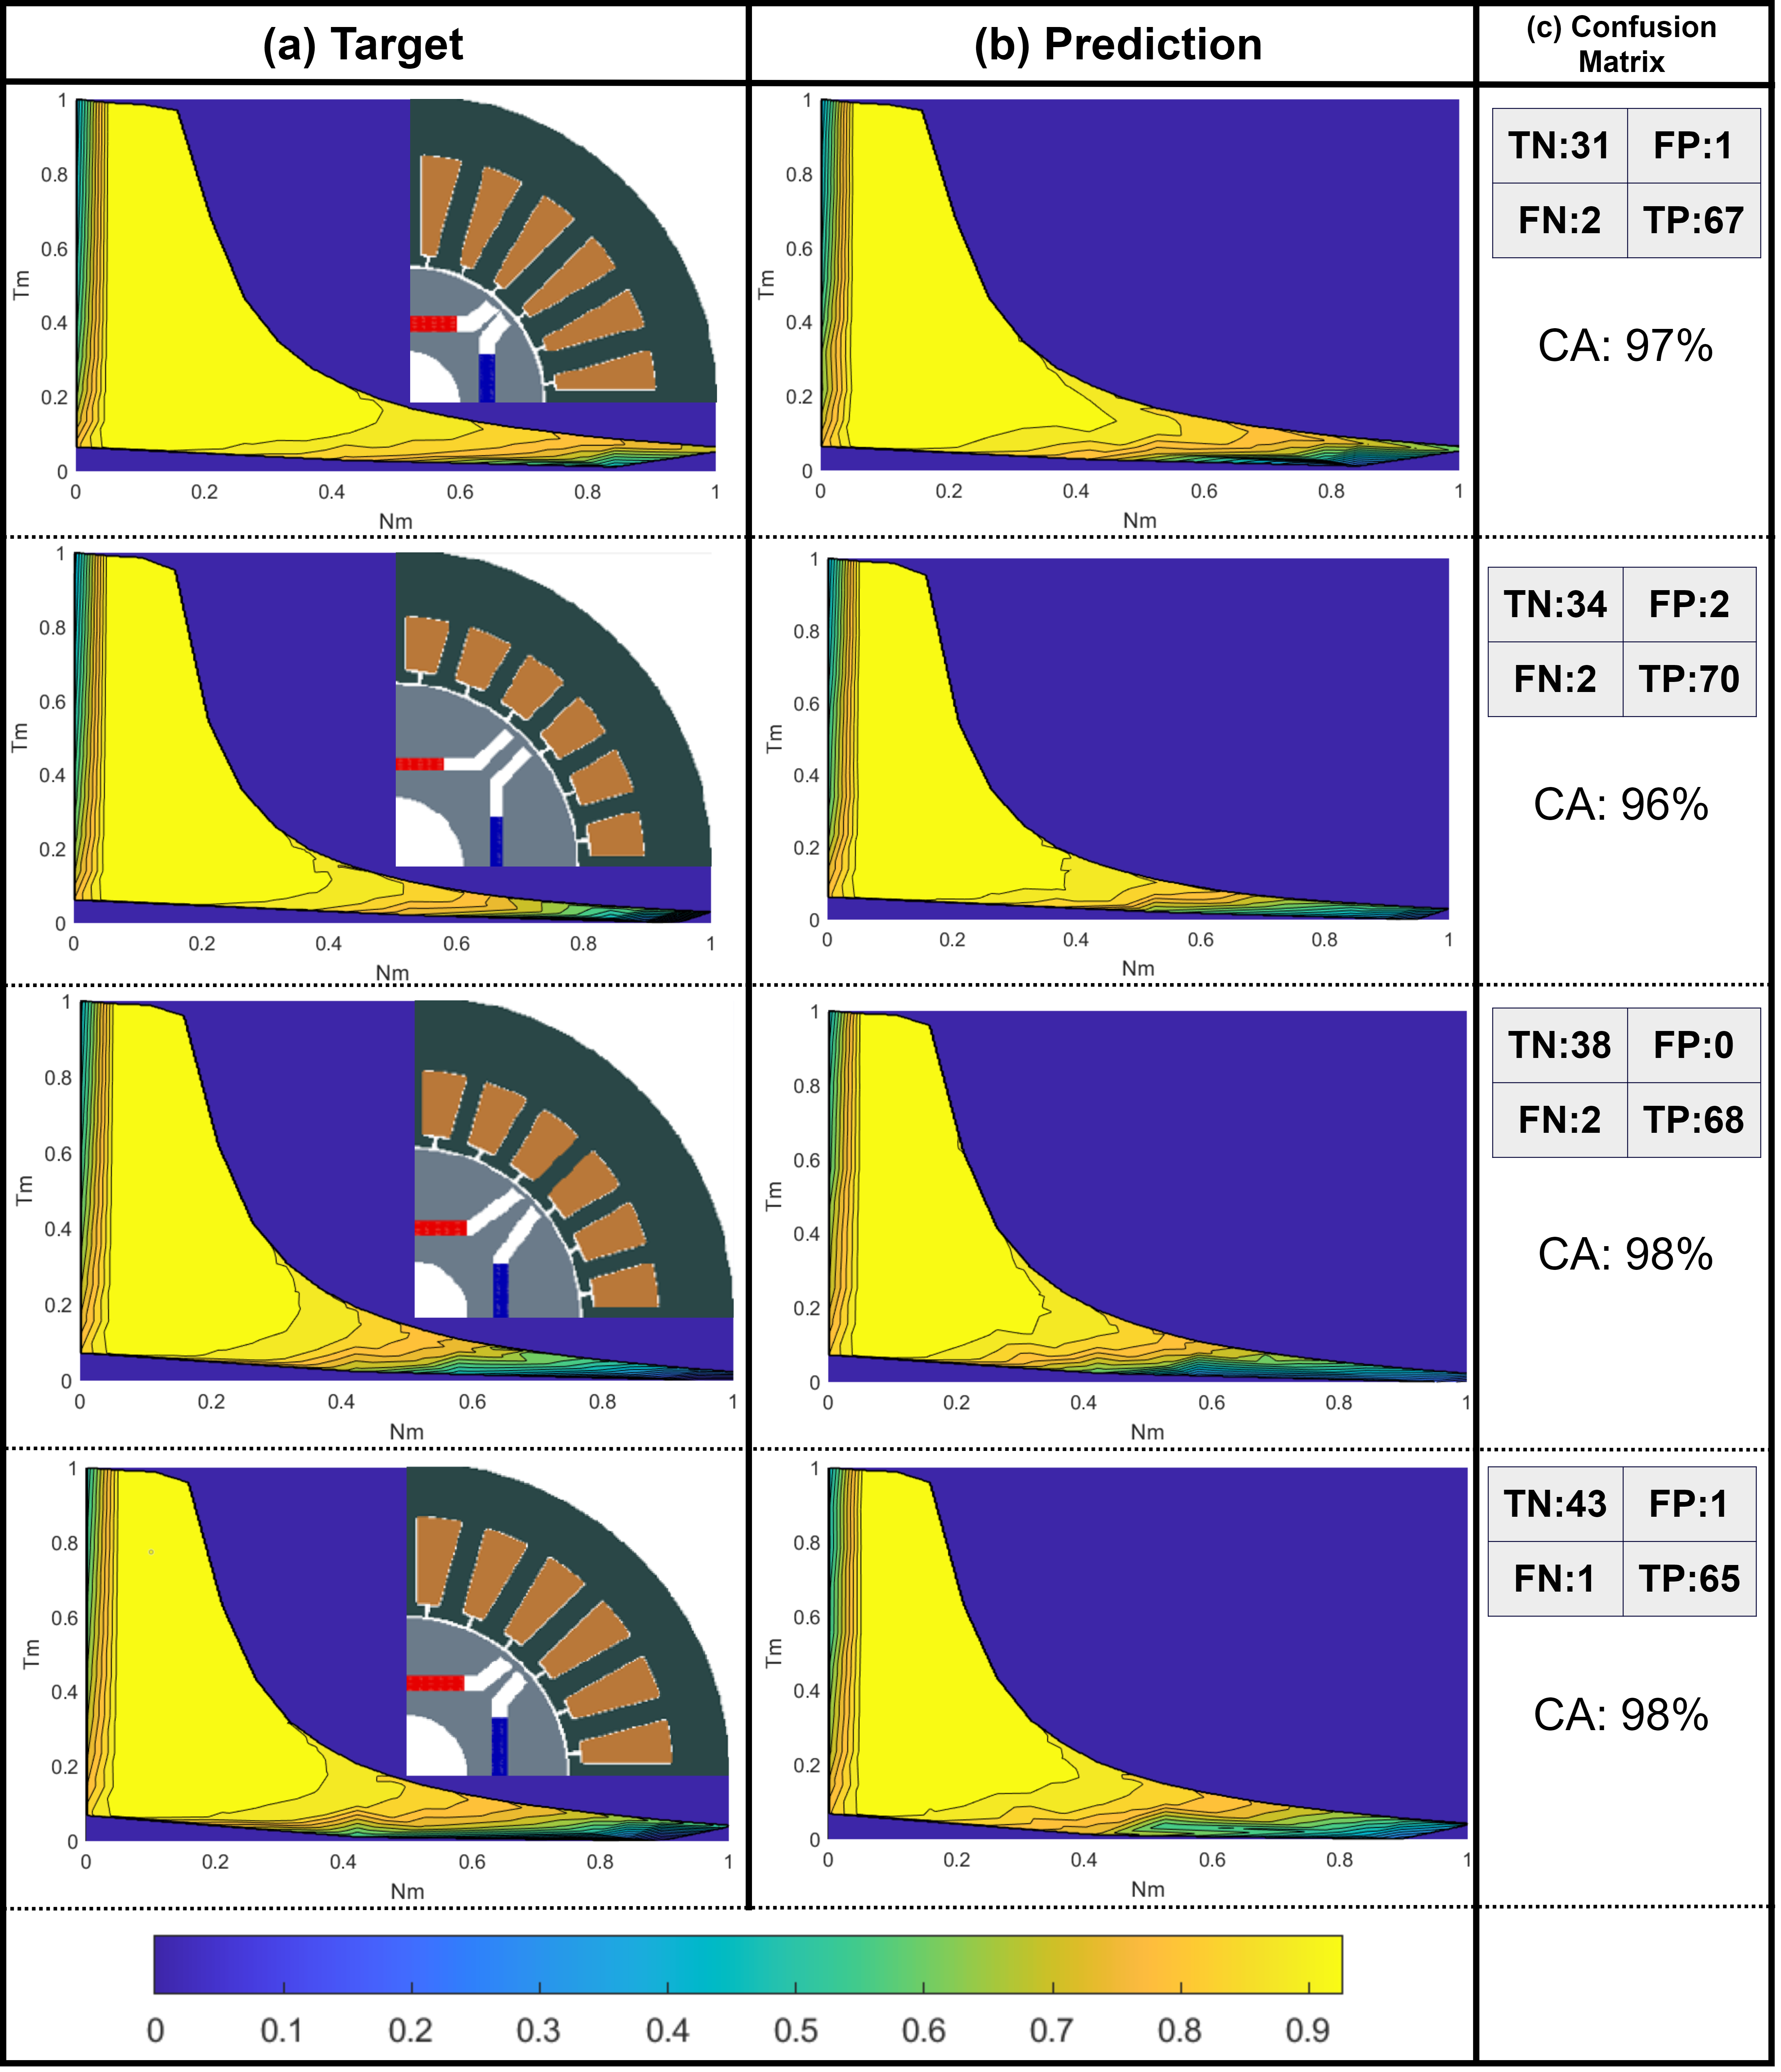
\includegraphics[width=\textwidth]{Figures/Chp_RNN/Qualitative_and_quantitative_results_Eff3.png}
    \caption{Qualitative and quantitative results of efficiency maps for two design samples: (a) Targets, (b) Predictions, (c) Confusion Matrices.}
    \label{fig:RNN_Fig-6_resultsRNN}
\end{figure}

For a more quantitative measure, the concept of a confusion matrix \parencite{geron2019hands} is used as a performance evaluator. The efficiency values are partitioned into two classes based on a threshold chosen here as 85\%. The ($T_{em}^*,N$) points in the efficiency map either belong to class 1 ($\eta^*>85\%$) or class 0 ($\eta^*\leq85\%$). Based on this classification, the following metrics defined in Table \ref{tab:RNN_confusionMatrix}, were used where CA is the classification accuracy in eqn. \ref{eqn:RNN_CA}. The variation of CA over 100 randomly selected designs from the test set is between 90-96\% indicating high accuracy in detecting high-efficiency regions in the tested maps. Since class imbalance is not an issue for this analysis, further measures derived from confusion matrix such as precision and recall are not evaluated.

\begin{table}[h!]
\centering
\resizebox{0.65\textwidth}{!}{%
\begin{tabular}{l||l|l}

                   & \textbf{Prediction: 0} & \textbf{Prediction: 1} \\ \hline \hline
\textbf{Target: 0} & True Negative (TN)     & False Positive (FP)    \\ \hline
\textbf{Target: 1} & False Negative (FN)    & True Positive (TP)     \\ \hline
\end{tabular}%
}
\caption{Confusion Matrix for high efficiency classification.}
\label{tab:RNN_confusionMatrix}
\end{table}

\begin{align}
    \text{Classification Accuracy} = \frac{TP + TN}{TP + TN + FP + FN} \label{eqn:RNN_CA}
\end{align}
The results presented were based on a dataset of 2900 samples used here as a proof-of-concept. Several constraints in terms of regularization and early stopping \parencite{caruana2001overfitting} were employed to check over-fitting during the training process. The network was trained on an NVIDIA 1050 Ti GPU and took around 5 mins per epoch with a batch size of 32. Convergence was achieved in around 25–35 epochs, resulting in a total run time of 2–3 hours. The prediction time is in the range of 10–12 seconds for 100 geometries at a time (batch size) which demonstrates an improvement over using FE simulations for this IPM motor. It should be noted that the time required to analyze multiple geometries is memory-bound rather than compute-bound, i.e. it is possible to parallelize the training and inference to thousands of samples if the memory requirements are satisfied. In comparison FE based calculation of an efficiency map can take between 1-2 hours, resulting in months to generate a dataset of this size. Further, the FE calculation is usually compute-bound. 

\subsection{End-to-end network approach}

Similar to the above, the end-to-end network was trained on the same GPU and took around 10 mins per epoch with a batch size of 16. The network converged in around 40–50 epochs with a total run time of 6–7 hours. The prediction time is in the range of 2–3 seconds for 100 geometries. Figure \ref{fig:RNN_Fig-8_resultsCNN} shows the target and predicted efficiency map for a sample IPM motor. The average mean squared error between the ground truth and the prediction lies in the range of 1-1.5\% per node/point in the 2D grid for a sample, similar to the performance obtained with the Modular network approach (Section \ref{sec:RNN_modular_results}).

A computationally cheaper surrogate for the time-consuming task of generating an efficiency map can streamline the process of design and analysis. However, a neural network will make a prediction even if the input is completely unrelated to what it has been trained on. A motor geometry significantly different from the ones in the training set can produce substantial errors. This creates a dilemma for the user; whether to trust the prediction or not in the absence of ground truth (FE results). To rely on such a predictor (trained in a supervised manner), it is necessary to provide an uncertainty measure in the results to quantify the confidence level. One way to achieve this is to extend the DL model using a probabilistic component in the neuron weights. The mathematical study on the theory of MC dropout can be found in Section \ref{section:CNN_MC_theory}.

\begin{figure}[h!]
    \centering
    \includegraphics[width=\textwidth]{Figures/Chp_RNN/Fig 7.png}
    \caption{Training curves for supervised efficiency map prediction.}
    \label{fig:RNN_Fig-7_trainingCurves}
\end{figure}

\begin{figure}[h!]
    \centering
    \includegraphics[width=0.75\textwidth]{Figures/Chp_RNN/Fig 8.png}
    \caption{End-to-end model: (a) Target, (b) Prediction.}
    \label{fig:RNN_Fig-8_resultsCNN}
\end{figure}

\begin{figure}[h!]
    \centering
    \includegraphics[width=\textwidth]{Figures/Chp_RNN/Fig 9.png}
    \caption{(a) Normalized error distribution, (b) Normalized uncertainty map}
    \label{fig:RNN_Fig-9_resultsMCDropout}
\end{figure}

Similar to Chapter \ref{chapter:2_CNN}, Monte Carlo (MC) dropout technique is used to quantify the uncertainty in the predictions. A high value of uncertainty  is an indicator that the designer should not rely on the prediction and perhaps employ conventional FE solvers instead. The error distribution, normalized for better visualization, over the efficiency map in Figure \ref{fig:RNN_Fig-8_resultsCNN} can be observed in Figure \ref{fig:RNN_Fig-9_resultsMCDropout} (a) and is highest around the edges of envelopes. A normalized uncertainty map for the same design sample using MC dropout implementation is shown in Figure \ref{fig:RNN_Fig-9_resultsMCDropout} (b). It can be seen that the  Bayesian approach could relate the regions of high error with high uncertainty. These uncertainty maps are computed by retrieving ten-MC samples from the network and calculating the standard deviation over the samples.

\section{Challenges with Supervised Learning}\label{RNN:6_Challenges_SL}

By learning a representation of the efficiency map, the various models in Section \ref{RNN:4_Neural_networks} can act well as a surrogate to FE simulations for geometries similar to the training data. However, a significant bottleneck throughout this work was the computational resources required to generate the training data. The data collection process took a total of more than 2 months, with four instances of motor design space being analyzed at a time using a FE software \parencite{mentor_motorsolve}. This is a major drawback of training an entire DNN from scratch (e.g. through random initialization). It is important to find a solution to this issue of the requirement that sufficient data for training is available from the same distribution. 

A possible solution to reduce the computational burden on both fronts (data generation and training time) is to use the concept of ‘transfer learning’ (TL) \parencite{pan2009survey}, where useful knowledge is extracted from neural networks trained on similar domains, i.e. motor geometries. The predictor for a new task will start its learning based on the knowledge extracted from a related task that has already been learned \parencite{mou2016transferable}. In other words, a pre-trained network, which is initially ill-prepared for the new task, is selected to make predictions and its network architecture is incrementally modified to fit the needs of the new task. This learning concept is necessary since many different motor configurations are available, and it will be impossible to generate massive datasets for all of them. Also, a model trained on one type of geometry can be used in creating a surrogate for other performances such as power factor and loss maps. Therefore, the following sections investigate transfer learning to reduce the training time of deep neural networks applied to electric motor drives by transferring knowledge over similar tasks. Two types of synchronous AC machines are studied: an interior permanent magnet (IPM) \parencite{khan2019deep} (the same as one used in Section \ref{RNN:3_dataCollection}) and a fractional-slot concentrated winding permanent magnet (FSCW PM) \parencite{reddy2012comparison, rahman2017comparison}. Design spaces of motor geometries are fed as inputs to the DNNs, which then output performance maps of motor drives, such as efficiency and power factor, as described below.

\section{Transfer Learning Methodology}\label{RNN:7_TL_methodology}

\subsection{Dataset Generation}

The technique for data generation is similar to that employed in Section \ref{RNN:3_dataCollection}. Different datasets of motor designs and performance maps are needed for the transfer learning problem. Each parameter of the reference designs in Figure \ref{fig:RNN_Fig_1} was varied by ±50\% of the nominal value. Next, Latin Hypercube sampling was used to generate a design space of 3200 samples for the parameterized PM motors. From these generated samples, 2500, 200, and 200 were randomly partitioned for the training, validation, and test sets, respectively. The additional (300) samples of the PM motor were not used for the TL process (Section \ref{RNN:9_Results_TL_Internal} \& \ref{RNN:9_Results_TL_External}) and act as a ‘data sufficiency’ check for Section \ref{RNN:9_Results_TL_DataRequirements}.

To calculate the performance maps, i.e. efficiency and power factor, a similar procedure as in \ref{RNN:3_dataCollection} and \parencite{mohammadi2017computational, khan2020efficiency} is adopted as shown in Figure \ref{fig:RNN_Fig_2}. For a given motor geometry and a set of parameters, electromagnetic finite element (FE) simulations \parencite{mentor_motorsolve} are run at various dq currents for motor characterization. Different motor control strategies are then solved to find the optimal excitation conditions for every speed. These points are used to compute optimal electromagnetic quantities, including torque, efficiency, and power factor, using FE simulations. Finally, the desired performance map is generated in the post-processing stage. Here, two DNNs were used to act as surrogates for the FE analysis, namely for Stages 1 and 3 of Figure \ref{fig:RNN_Fig_2}.
\\

\begin{comment}
\begin{figure}
    \centering
    \includegraphics[width=0.25\textwidth]{Figures/Chp_RNN/Fig_1b.png}
    \caption{Caption}
    \label{fig:my_label}
\end{figure}
\end{comment}

\begin{minipage}{\textwidth}
  \begin{minipage}[b]{0.4\textwidth}
    \centering
    \includegraphics[width=0.85\textwidth]{Figures/Chp_RNN/Fig_1b.png}
    \captionof{figure}{Parametrized Motor Geometry of FSCW PM Motor}
    \label{fig:RNN_Fig_1}
  \end{minipage}
  \hfill
  \begin{minipage}[b]{0.59\textwidth}
    \centering
    \begin{tabular}{||c||}\hline
      Independent Parameters \\ \hline \hline
        12 slots \hspace{20pt} 10 poles \\
        300 A_{rms} \hspace{10pt} 450 V_{dc} \\ \hline \hline
    \end{tabular}
    \centering
    \begin{tabular}{||c|c||c|c||}\hline
      Parameter & Value & Parameter & Value \\ \hline \hline
        $X_1$ & 13 mm & $X_6$ & 115 mm\\
        $X_2$ & 25 mm & $X_7$ & 122.5 mm\\
        $X_3$ & 4.3 mm & $X_8$ & 12.5 mm\\
        $X_4$ & 7 mm & $X_9$ & 60 mm\\
        $X_5$ & 1.0 mm & $X_{10}$ & 0.25 mm\\ \hline
      \end{tabular}
      \captionof{table}{Dependent \& Independent Parameters of the reference design for a FSCW PM Motor}
    \end{minipage}
  \end{minipage}
  
\subsection{Problem Definition of Transfer Learning} \label{RNN:7.2prob_def_TL}

Transfer Learning is a well-studied topic in the field of machine learning. This work focuses on performing model-based knowledge transfer, which is the most popular methodology for DNNs \parencite{pan2009survey}. The main aim is to enhance the ‘generalizability’ of DNNs, which is necessary to reduce the future costs of training networks on similar tasks and at the same time improve the network’s robustness. The magnitude of similarity between two ML tasks is not a well-defined metric but an attempt can be made by relating the input features and the label space of the task. Using the notation defined in \cite{pan2009survey}, the task of prediction using a ML model can be seen as a representation of the domain to the target label. The domain ‘D’ is composed of two components: a feature space X and a marginal probability distribution $P(x)$, where each input observation in the dataset belongs to X, i.e. $x \in X$. For a given domain, a label space ‘$L$’ also has two components $Y$ and $P(y | x)$, where the probabilistic function denoted by $P(y | x)$ can make predictions on instances from $X$. In the case of \parencite{khan2020efficiency}, the labels were efficiency values for each design point and a design point was represented by the geometrical features (either as CAD image or design vector) and the excitation points. For supervised learning, we require data for a domain and corresponding data for labels. On the other hand, for TL, a model must be trained on a source domain and labels $(D_s,L_s)$ and also on target data for the domain and labels $(D_t,L_t)$ where the original knowledge is to be transferred. 
This work explores knowledge transfer capability over two scenarios as shown in Figure \ref{fig:RNN_Fig_3}. In the first scenario, the source task of efficiency map prediction estimation is replaced with the target task of a power factor map, over the same IPM geometry. In this case the source and target domain remain the same $(D_s=D_t)$, but the label space changes ($L_s \neq L_t$). For the rest of the Chapter, this task will be referred to as ‘Internal Knowledge Transfer’. 
On the other hand, the task referred to as ‘External Knowledge Transfer’ involves the prediction of efficiency maps but over a different design space of a FSCW Surface-mounted PM motor. This is a comparatively less similar task since neither the domains nor the labels necessarily overlap ($D_s \neq D_t$ and $L_s \neq L_t$) completely. However, given the domain spaces ($D_s,D_t$), there can be some resemblance over the labels since both $Y_s$ and $Y_t$ are bounded between 0-100\% and the conditional probabilities can also be relatable. Calculating performance maps remains the same based on the domain knowledge. Understanding the source and target task is important as it was observed that very dissimilar tasks fail in the transfer learning process \parencite{mou2016transferable}.

\begin{figure}[h!]
    \centering
    \includegraphics[width=\textwidth]{Figures/Chp_RNN/Fig_2.png}
    \caption{Flowchart of the process for calculating performance maps.}
    \label{fig:RNN_Fig_2}
\end{figure}

It is also important to distinguish TL from a closely related learning paradigm called multi-task learning. Although both aim to generalize and exploit the common knowledge shared by different tasks, the approaches are different. TL focuses on learning a new task using some source task as auxiliary information. Conversely, multi-task learning tries to jointly improve the general performance of all the constituent tasks without any source or auxiliary information. As such, multi-task learning requires training data for all the tasks to be learned. The goal of multi-task learning is not to reduce the data dependency or the computational load. This also highlights the advantage of TL in cases where the source pre-trained model has millions of weight parameters and is trained on massive datasets that needed significant GPU hours. Access to only the trained weights along with the network architecture is needed for transferring knowledge to a target task.

\subsection{Knowledge Transfer Procedure}
After identifying the source and target tasks, the next step is the procedure of transferring the knowledge from the source to the target. Only Stage 3 of Figure \ref{fig:RNN_Fig_2} is used here for TL, since the data and computation required for Stage 1 was significantly lower than that for Stage 3, i.e. Stage 1 can be trained in a supervised manner. The source training data remains the same, as used in Section \ref{RNN:3_dataCollection} to train the network in Section \ref{RNN:4_Neural_networks}.
For Stage 3, the general approach used to achieve successful transfer of knowledge is by combining the techniques of greedy pre-training followed by fine-tuning the overall model. The idea of greedy layer-wise pretraining is widely used in training deep belief networks and autoencoders \parencite{goodfellow2014generative}. However, the DNN weights, in this case, are trained in a supervised manner. A certain part of the pre-trained network is identified as prior knowledge, which is useful for the new task and can be identified as the common knowledge between the source and target task. Greedy pre-training ‘freezes’ the prior knowledge part of the pre-trained network and substitutes the rest of the network with corresponding ‘new’ layers. The terms ‘frozen’ and ‘new’ refer to whether the gradient can flow through the layers during training through backpropagation. A ‘frozen’ layer will not see a change in its weights during the training procedure, whereas a ‘new’ layer, initialized either randomly or using one of the initialization techniques \parencite{goodfellow2014generative}, is trained in a supervised manner during the pre-training stage.

\begin{figure}[h!]
    \centering
    \includegraphics[width=\textwidth]{Figures/Chp_RNN/Fig_3.png}
    \caption{Transfer learning tasks: Internal Knowledge Transfer (IPM to IPM) and External Knowledge Transfer (IPM to PM).}
    \label{fig:RNN_Fig_3}
\end{figure}

Once the new layers are sufficiently trained and are assumed to work in synchronization with the ‘frozen’ or prior section of the network, the whole network is fine-tuned. This process is similar to supervised learning, where the gradient flows through the whole network, making changes in the weights of all layers and no part of the network is in the ‘frozen’ state anymore. One distinction in practice is reducing the learning rate during the fine-tuning step, as large changes in the pre-trained part of the network can compromise the highly optimized weights from the source model. Although guidelines for the learning rate are not well defined, in this work the learning rate was reduced by an order of 10 between the greedy pre-training and fine-tuning step. 
Ideally, the pre-trained network must be retained as much as possible to leverage the powerful expressive ability of deep learning models. The decision to freeze or replace a part of a network is highly task-dependent and certain guidelines that were observed during this work are discussed next.

\section{Results of Transfer Learning}\label{RNN:9_Results_TL}
As explained earlier, transfer learning aims to decrease the computational load by reducing the data requirement and training cost on the target task. To compare the training time, supervised learning on the same target task serves as the benchmark. Once the ideal performance for a task is identified, the training data is systematically reduced until there is a significant drop in model performance and the data requirement threshold for successful knowledge transfer is saved.
To quantify the change in weights and to compare the relative change with other layers in the same network, the weight distribution of each layer from the pre-trained network is compared with the target network through a hypothesis test of statistical significance between the two means of the weights:

\begin{align}
    H_0 : \mu_s = \mu_t \\
    H_a : \mu_s \neq \mu_t
\end{align}

Here, the $\alpha$-value (coverage) is set to 0.05 or 5\%.

Instead of using classical formula based statistical methods for hypothesis testing, a resampling based technique is used (as described in Chapter 5, \cite{bruce2020practical}). The procedure behind this resampling based hypothesis test is to combine the data from both sets (pre-trained and trained weights) and repeatedly draw samples without replacement from the permuted data. On calculating the quantity of interest (difference in weights between the two sets), one can obtain the distribution due to random variation in the weights of the two NNs. Based on the hypothesis test, if there is no significant difference in the mean values of layers from the source and target model, then these layers are denoted by the ‘green’ color in Figure \ref{fig:RNN_Fig4a}. A p-value failing to cross the threshold results in failing to reject the null hypothesis, i.e. there is no significant difference in the mean values of both layers from source and target models. These insignificant layers are denoted by ‘green’ color in Figure \ref{fig:RNN_Fig4a}. The largest change in weights for a layer in the network is denoted by the color ‘red’. The level of change is relative to the change observed in other layers of the same network and all the changes in between the two extremes (‘red’ & ‘green’) are denoted with ‘yellow’ color. To quantify these changes, the architecture is kept the same between the source and target neural networks. No additional layers were added to the source network in this study.

\subsection{Internal Knowledge Transfer}\label{RNN:9_Results_TL_Internal}

To transfer part of the pre-trained network that was originally trained on efficiency maps to power factor maps, the domain remains the same ($D_s=D_t$), i.e. the same geometric variations of the IPM motor are used. Since the label space for the target is significantly different from that of the source, the output layer (time-distributed dense layer) of the pre-trained network was replaced with a new layer. The process of greedy supervised pre-training was used to train this layer with a learning rate of $1 \times 10^{-3}$. After sufficient training, the network was fine-tuned with changes performed in all layers at a learning rate of $1 \times 10^{-4}$. Overall, TL managed to save about 50-55\% in training time compared to a cold-start supervised learning process as shown in Figure \ref{fig:RNN_Fig5a}. All other configurations for using different parts of the network for pre-training and fine-tuning were tested and did not result in a better performance than the one shown in Figure  \ref{fig:RNN_Fig4a}. The majority of change in weights is observed in layers closer to the output, which matches with the discussion in Section \ref{RNN:7.2prob_def_TL}. Similar to \ref{RNN:5_Results_Discussion}, the normalized RMSE over the test set lies in the range of 0.25-1.0\% per point in the \textit{pf} map.

\begin{figure}[h!]
    \centering
    \includegraphics[width=\textwidth]{Figures/Chp_RNN/Fig_4a.png}
    \caption{Change in weights of each layer: Efficiency map to Power factor map (IPM to IPM)}
    \label{fig:RNN_Fig4a}
\end{figure}

\begin{figure}[h!]
    \centering
    \includegraphics[width=\textwidth]{Figures/Chp_RNN/Fig_5a.png}
    \caption{Comparison of training curves between supervised learning and transfer learning tasks: Efficiency map to Power factor map (IPM to IPM)}
    \label{fig:RNN_Fig5a}
\end{figure}

\subsection{External Knowledge Transfer}\label{RNN:9_Results_TL_External}

For the External Knowledge Transfer task, the difference mentioned in Section \ref{RNN:7.2prob_def_TL} lies with both the domain and label parts of the task, which differs from the original one. Also, the geometrical features do not match as seen in Figure \ref{fig:RNN_Fig_3}. Hence, the feedforward network must be modified completely with new dimensionality to match the input dimensions, but at the same time should work in tandem with the rest of the network. The rest of the network is tuned only after appreciable training is completed with the input part of the network. However as seen in Figure \ref{fig:RNN_Fig4b}, the changes in the network are distributed evenly near the input and output layers, signifying the hypothesis in Section \ref{RNN:7.2prob_def_TL}. The normalized RMSE value per point lies in the range of 2-3\%, which is slightly worse than that obtained for the IPM Motor in Section \ref{RNN:5_Results_Discussion} ($\approx 1.5\%$). As observed in the training curves of  Figure  \ref{fig:RNN_Fig5b} the computation load for training has been reduced by about 40-45\% as compared to a supervised learning approach on the same task. 

\begin{figure}[h!]
    \centering
    \includegraphics[width=\textwidth]{Figures/Chp_RNN/Fig_4b.png}
    \caption{Change in weights of each layer: Efficiency map to Efficiency map (IPM to PM).}
    \label{fig:RNN_Fig4b}
\end{figure}

\begin{figure}[h!]
    \centering
    \includegraphics[width=\textwidth]{Figures/Chp_RNN/Fig_5b.png}
    \caption{Comparison of training curves between supervised learning and transfer learning tasks: Efficiency map to Efficiency map (IPM to PM)}
    \label{fig:RNN_Fig5b}
\end{figure}

\subsection{Data Requirements}\label{RNN:9_Results_TL_DataRequirements}

The other significant contribution of TL is the reduction in the training data needed to successfully train a network. For this reason, part of the overall data is held out to check for ‘data sufficiency’ (300 samples). The remaining data is divided into the usual components of train, validation, and test parts for TL. The training data is continuously decreased until a significant drop in model performance is observed. This performance is observed over the ‘data sufficiency’ part of the dataset. This study yields the threshold of data required to successfully perform transfer learning on this task with this network. A grid search was performed with the percentage of data used for TL starting from 100\% and randomly removing 5\% of the data at each step of the search. With this study, it was observed that only 60-65\% of the data is needed for Internal Knowledge Transfer and about 75-80\% of the data needed for External Knowledge Transfer. This demonstrates that the more dissimilar the source and target tasks are in terms of either domain or label space, the more data will be needed for successful TL processes.

Multiple runs for each test (for TL tasks and Data sufficiency check) were performed with the random seed being the only difference.

\section{Conclusion}\label{RNN:10_Conclusion_TL}

This work shows that by learning a representation of the efficiency map, the various models in Section \ref{RNN:4_Neural_networks} can act as a surrogate to FE simulations with high accuracy, for geometries similar to the training data. For geometries significantly different from the training data, transfer learning was employed.
Transferring knowledge from one domain to another allows machine learning systems to extend their range of applicability beyond their original creation. Instead of training a neural network from scratch for every problem, transfer learning enables the reuse of models resulting in fewer computational resources being needed. The results demonstrated that for both case studies (i) the training time was reduced by more than 40\% and (ii) at most 80\% of the training data. This generalization ability also helps to make machine learning models more accessible and more robust in many areas where capabilities or resources such as computing power, data, and hardware might be scarce. Once two domains are known to be close to each other, deep neural network models can be propagated from a well-developed domain to a less-developed domain. Also, in situations that differ from the training data, the trained models need adaptation, before they can be used for the target task. 

Finally, it was also found that all the studied models predicted the efficiency maps with high accuracy, and with the advantage of GPUs and probabilistic methods, a parallelizable and robust method to produce efficiency maps is feasible.


\begin{comment}

\section{Transfer Learning}

For future,\textbf{ an extension which explores involving multi-task learning} with transfer learning can further reduce the computation burden


It is not a good idea to train a Deep Neural Network from scratch. This saves us time as instead of collecting enormous amount of data which is both a computationally expensive and time consuming task. Instead we can focus on finding a neural network that acompalishes similar task as compared to the one we are targeting. This technique is called transfer learning. We have a neural network that was trained on efficiency maps of a IPSM and we have another task which is similar one but has a different geometry. Thus saving time and computational resources on both front. These tasks are very similar and even partially overlapping, so we should try to reuse the parts of the network.


\subsection{Definition \& Problem Formulation}

\subsection{Historical Findings}

\section{Explain Problem}

\subsection{Two problems that I have}

\subsection{CNN fine tuning and RNN fine tuning}

\section{Architecture Explanation}

\subsection{Original architecture being used}

\section{Results}

\subsection{Training Time}

\subsection{Table for layer changes}

\subsection{Amount of Data needed
}












Further we have another task where we try to predict a different performance parameter. The level of similarity exceeds here since the input is infact overlapping. This encourages a source to reuse parts of the network to use for these new two tasks. 

Why geometric information might not be ideal?

If the input dimensionality of the new task is not the same as the input dimensionality of the original task, we can add some pre-processing step to resize them to the size expected by the original model. However trasnfer learning works best when inputs have similar low-level features. 

Changes to the model.
The output layer of the original model should be replaced because it is most likely not useful for the new task. The usual practice of transfer learning preserves the lower level layers and focuses on the upper level. \textit{Clarify lower and upper}. The closer a leyer is to the output of the network, the upper it is considered. 

Further if there is significant similarities between the tasks, then the outer layer can be preserved and some additional layers can be added to handle for a more complex task. 

In another scenario, the network does not encounter a architectural change and is simply re-trained.

The re-training is different from the usual training and is described in th next section. 

The upper hidden layers of the original model are less likely to be useful as the lower layer since high level features that are most applicable for the new task may differ significantly from the ones that were most rewarding for the original task. All of this is very subjective. Since we have a lot of choices here, it is important to use domain knowledge to use the prioor knowledge to ocus on the startegies that are highly relevant to work well.

Bascically the more similar the tasks are, the more layers we want to reuse (starting from the lowest)

To keep a layer ouyt of training, we freeze the reused layers firstr ie make the weights untrainable during the backpropagation stagte. So that stochastic optimization will jnoyt modify the fine tuned weights,.

As a rule of tump, the more training data we have the more layers can be unfrozed or more layers can be added to the pre-existing network. Also we can reduce the learning rate when unfreezing reused layers. This will limit the amount of change to the otherwise fine-tuned weights. 


\section{Conclusion}

\section{Introduction}

% 3A
How learning algorithms can acquire information/knowledge about the tasks outside the source domain. 
% 4A
Even though a machine learning model can be made to be of high quality, it can also make mistakes, especially when the model is applied to different scenarios from its training environments. 
% 4B
The decision making capability can significantly drop-off. 
% 4C
This is because model trained by machine learning algorithm can be outdated and needs updating when new situation occurs.  It is this need to update or transfer models from one scenario to another that lends importance to the topic of this work.
% 4D
a major challenge in practicing machine learning in many applications is that models do not work well in new task domains. Lack of new training data due to the small data challenge, changes of circumstances and changes of tasks. 

% 4d.2
Machine learning models cannot do well without sufficient training data. Obtaining and labeling new data often takes much effort and resources in a new application domain

Challenges of this work:

\begin{enumerate}
    \item Small data.
    \item Change of circumstances.
    \item Change of task.
\end{enumerate}

% 5A
In situations that differ from the training data, the trained models need adaptation before they can be used

% 5B
In a nutshell, transfer learning refers to the machine learning paradigm in which an algorithm extracts knowledge from one or more application scenarios to help boost the learning performance in a target scenario. 

% 5C
data sparsity and cold start problems in many large-scale and online applications 

% 6A
Based on the transfer learning methodologies, once we obtain a well-developed model in one domain, we can bring this model to benefit other similar domains. Hence, having an accurate “distance” measure between any task domains is necessary in developing a sound transfer learning methodology
If two domains are closely related, transfer learning can be fruitfully applied.

% 6B ------- Conclusion/ Justification
Once we know that two domains are close to each other, we can ensure that AI models can be propagated from a well-developed domains to less-developed domains

%6C  ------- Conclusion
Being able to transfer knowledge from one domain to another allows machine learning systems to extend their range of applicability beyond their original creation. This generalization ability helps make AI more accessible and more robust in many areas where AI talents or resources such as computing power, data and hardware might be scarce.


% 6D History

Transfer learning has been studied under different terminologies in AI, such as knowledge reuse and CBR, learning by analogy, domain adaptation, pre-training, fine-tuning, and so on.
In particular, transfer of learning refers to the process in which past experience acquired from previous source tasks can be used to influence future learning and performance in a target situation.
transfer of learning in education tries to study how humans adapt in education, the processes or algorithms of transfer are similar.

% 7A
We define what “domain,” “task” and “transfer learning” mean by following the notations introduced by Pan and Yang (2010). For [Compumag], the domain was the inputs in the form of geometrical and excitation. The domain `D' is composed of two components: a feature space X and a marginal probability distribution $\mathdc{P}X$ , where each input instance of the dataset belongs to X ($x \in X$).
% 7B
For a given domain, D = {X ,PX }, the task T will have two components: the target space Y and a probabilistic function P(y|x), which can make predictions on instances from X. For [Compumag], the labels were efficiecny values for each design point in the Torque-Speed map.
If two domains differ, it can be either due to difference in the feature space or the marginal probability distribution.

% 7C
So following the terminology from [Pan], We have identified a source domain Ds and learning task
Ts, a target domain Dt and learning task Tt. 
For this work, we focus on two different scenarios as shown in Fig ..., where in the first task called `Internal knowlwdge transfer' where the domain is the same, but there is a difference in the task to be performed $D_{s1} = D_{s2}$ and $T_{s1} \neq T_{s2}$. On the other hand the second task can be called as `External knowledge transfer' where there is a deffinete difference in the source domain and a possible difference in the task as well.  $D_{s1} = D_{s2}$ and $T_{s1} \neq T_{s2}$. Here the range of the task will probably be the same but there is a definite difference between the conditional probability 

% 8B
The main aim of transfer learning is to counter the lack of training data problem in target domain with more knowledge gained from the source domain.

%
Most of the literature on transfer learning focuses on the different techniques related to what part of the network or the methodology of the transfer. An understanding of ideal scenario of when to transfer knowledge is equally important is left at the discretion of the domain expert to decide. An ideal scenario would be when either of domain or the task share some commanility. In this case, internal knowl;edge transfer has the domain being the same both in terms of the range and distribution. For the other case, we know that the range is not the same, but some relation on the conditional probablity can be exploited. 

% 11 A
The main aim is introducing `generalization'. ML models should be robust and general enough that apply not only on training data but relevant data that is closely represented. TL tries to generalize commonalities across different tasks and domains. This difference makes transfer learning an important part in the world of ML.

%12 A
One of a closely related learning paradigm to transfer learning is multi-task learning.  

Although both transfer learning and multitask learning aim to generalize commonality across tasks, transfer learning is focused on learning on a target task, where some source task is used as auxiliary information, while multitask learning aims to learn a set of target tasks jointly to improve the generalization performance of each learning task without any source or auxiliary tasks.

As most existing multitask learning methods consider all tasks to have the same
importance, while transfer learning only takes the performance of the target task
into consideration, some detailed designs of the learning algorithms are different. 

Transfer Learning holds advantage over multi-task learning in cases where only the trained model is available and not the source training data. Further, since model transfer learning uses the source model as a starting point, they tend to train faster than a cold start multi-task learning process.

% 45 A
Although there are different ways to transfer relevant information from ML model to another assuming that the source task and the target task share some common knowledge in the model level.

% 45 B
model-based transfer learning leverages the knowledge in the source domain

% 45 C
The model based training depends on the assumption that the source model has learned a lot of the structure from the data. Using this structure on a related target task, this knowledge is transferred top learn a more precise target model and obtain a more powerful model that can be obtained using only limited training data.

% 45 D TL vs Multi
multitask learning tries to optimize the performance on a lot of target tasks simultaneously, while transfer learning only focuses on improving the performance of one target domain by exploiting knowledge from auxiliary task

% 46 A
establish the target model by reusing some components in the source model or
reusing some hyperparameters of the source model

% 47 A
Shared model components can serve as prior knowledge that can help train the new layers in the network. This way once we achieve sufficient pre-training of the layers, the whole model can be unfrozen to continue training onwards.

% 47 B
Once we apply a prior like this, we can obtain a model of satisfactory performance even with limited training data on the target task.

% 49 A

We try to focus on leveraging the powerful expressive ability of deep learning models to extract and transfer knowledge which can relate to both the source and target domain and task.

% 54 A
Parameter fine-tuning is a simple and effective technique for knowledge transfer in terms of model parameters

For transfer of knowledge between two different types of motors, the geometrical representation differs significantly both in terms of number of parameters and thus the input differs both in terms of dimensionality and meaning corresponding to each geometrical parameter. There was not a difference in excitation representation for RNN input. The idea of greedy network pre-training is performed, where 


The idea of greedy layer-wise pretraining has been widely used in training deep belief networks and autoencoders. In this approach, the parameters trained using unsupervised learning are used to initialize specific classification tasks (Bengio, 2012). 

This approach assumes that unsupervised learning tasks such as instance
reconstruction can reveal good representations. 

The parameters initialized with them should be in a good region for the downstream tasks. Such initialization strategy can be considered as a kind of regularization on the learned model parameters.

% 54 D

The second stage is fine-tuning with supervised learning where the model weights are  
\end{comment}